\chapterimage{WaterPumpingCover}
\chapter{Pumping Systems}




\begin{table}[H]
\begin{tabular}{| m{1cm} | m{15cm} |}
\hline
\multicolumn{2}{|l|}{\textbf{Expected   Range of Knowledge for Water Properties and Sources}}                                                                          \\ \hline
\multicolumn{2}{|l|}{\textit{Water   Distribution System Operator License Exams}}                                                                                      \\ \hline
D1 & Ability to read   and interpret a pressure gauge                                \\ \hline
D1 & Ability to recognize   abnormal pressure readings (too high or too low)         \\ \hline
D1 & Ability to recognize   abnormal pump operating conditions                       \\ \hline
D1 & Knowledge of pump   types                                                       \\ \hline
D1 & Knowledge of the   relationship between water velocity and water pressure       \\ \hline
D2 & Ability to repair and   replace pump and motor system components                \\ \hline
D2 & Knowledge of   operational principles of a water pump                           \\ \hline
D2 & Knowledge of packing   gland settings                                           \\ \hline
D2 & Knowledge of pump   maintenance procedures                                      \\ \hline
D2 & Knowledge of the   mechanical components of pumps and motors                    \\ \hline
D2 & Knowledge of the   relationship between head loss and friction                  \\ \hline
D3 & Ability to interpret   a pump curve                                             \\ \hline
D3 & Ability to match pump   type to application                                     \\ \hline
D3 & Knowledge of proper   phase balance                                             \\ \hline

\end{tabular}
\end{table}
\newpage



\begin{table}[H]
\begin{tabular}{| m{1cm} |m{15cm} |}
\hline
\multicolumn{2}{|l|}{\textbf{Expected   Range of Knowledge for Water Properties and Sources}}                                                                      \\ \hline
\multicolumn{2}{|l|}{\textit{Water   Distribution System Operator License Exams (Continued)}}                                                                  \\ \hline
D3 & Knowledge of proper   pump alignment                                            \\ \hline
D3 & Knowledge of   recordkeeping requirements                                       \\ \hline
D3 & Knowledge of the   effect of corrosion on head loss                             \\ \hline
D3 & Knowledge of when to   "MEG" a motor                                            \\ \hline
\multicolumn{2}{|l|}{\textit{Water   Treatment Operator License Exams (Continued)}}                                                                  \\ \hline
T1 & Ability to   discriminate between normal and abnormal operation of a water pump \\ \hline
T1 & Knowledge of pump   types and uses                                              \\ \hline
T1 & Knowledge of the   components of a water pump                                   \\ \hline
T1 & Knowledge of the   operation of a water pump                                    \\ \hline
T1 & Knowledge of valve   types and uses                                             \\ \hline
T1 & Ability to replace   components of a water pump                                 \\ \hline
T2 & Knowledge of pump   installation procedures                                     \\ \hline
T3 & Ability to administer   a safety plan                                           \\ \hline
\end{tabular}
\end{table}
\newpage



\section{Background}\index{Pumps!Background}

\begin{itemize}
  \setlength\itemsep{1em}
\item A pump is a device that inputs energy into the water to increase its pressure and/or increase its flow.  Pumps typically convert electrical energy into hydraulic energy of the water.  

\item For water treatment and distribution, pumps are widely used for purposes which include the following:

\begin{itemize}
  \item Remove water from a source, such as a river, lake, reservoir, well, spring, or muskeg pond.

  \item Move water from the treatment plant to the distribution system or reservoir.

  \item Circulate water through a distribution system.

  \item Maintain pressure in the distribution system.

  \item Pump chemicals into the system.

\end{itemize}

\begin{figure}[H]
\begin{center}
\includegraphics[scale=0.7]{PumpTypes1}
\caption{Pump Types}
\end{center}
\end{figure}


\item Pumps can be classified as: 
\begin{enumerate}
\item Rotodynamic pumps:  Here the energy is continuously imparted to the pumped fluid by means of a rotating impeller, propeller or rotor. 



These pumps transfer mechanical energy to the fluid primarily by increasing the fluid kinetic energy. Kinetic energy is then converted into potential energy (pressure) in the discharge collector. 

\vspace{0.2cm}

The most common types of rotodynamic pumps are:
\begin{itemize}
\item Radial (centrifugal)
\item Mixed flow, and 
\item Axial flow (propeller) pumps - vertical turbine pumps.
\end{itemize}

\begin{figure}[H]
\begin{center}
\includegraphics[scale=0.35]{TypesofRotodynamicPumps}
\caption{Types of Rotodynamic Pumps}
\end{center}
\end{figure}

\item Positive-displacement pump: These pumps utilize a mechanical device such as a piston or plunger to pump the fluid.
\end{enumerate}

\end{itemize}
\section{Rotodynamic pumps}\index{Pump type!Rotodynamic pumps}
With this pump, the volume of the liquid delivered for each cycle depends on the resistance offered to flow. A pump produces a force on the liquid that is constant for each particular speed of the pump. Resistance in a discharge line produces a force in the opposite direction. When these forces are equal, a liquid is in a state of equilibrium and does not flow. If the outlet of a non-positive-displacement pump is completely closed, the discharge pressure will rise to the maximum for a pump operating at a maximum speed.
\subsection{Centrifugal pumps}\index{Pump type!Centrifugal pumps}

\begin{itemize}
\item Centrifugal pumps are the most common type of pump used in water systems. 

\item In a centrifugal pump, energy is transferred from the shaft to the impeller and from the impeller to the water.

\item Centrifugal force - the force used to throw the water from the spinning impeller in a centrifugal pump, is the same force that is experienced by the ball when whirled on a string.

\item The centrifugal pump components related to imparting the energy to the water include:

\begin{itemize} 
\item Volute - Also called casing, it surrounds the impeller.  Its spiral-like geometry with an increasing through-flow area, reduces the impeller induced fluid velocity and increases its static pressure. The fluid exiting the casing is then diffused towards the casing discharge.

\item Impeller - A rotating set of vanes designed to impart rotation to a mass of fluid.  flow enters the impeller which is in line with the pump shaft but the flow exits from the impeller perpendicular to the pump shaft.

\begin{figure}[h!]
\begin{tabular}{  m {8cm}  m {8cm}} 
\begin{center} \includegraphics[scale=0.3]{CentrifugalPumpOperatingPrinciple} \end{center} & \begin{center}\includegraphics[scale=0.25]{CentrifugalPumpCase} \end{center} \\
\multicolumn{2}{c}{\textit{Centrifugal Pump Operating Principle}}\index{Centrifugal pumps!Operating principle}                                                                \\\\
\end{tabular}\\
\end{figure}
\item Water being pumped provides cooling to dissipate the heat generated by its moving parts - shaft and impeller.  If the pump is run dry for an extended period of time, the heat generated may severely damage to the pump and greatly limiting its service life.
\end{itemize}

\end{itemize}
\subsubsection{Centrifugal Pump Types}\index{Centrifugal pumps!Types}                                                               
\begin{enumerate}
\item One way to classify impellers is based on the use a or lack of shroud or covering. 
\begin{itemize}
\item Closed impeller: This impeller has a top and bottom shroud and is used in large pumps primarily in clean water pumping application as it is prone to clogging when in contact with solids.
\item Open impeller:  Here the vanes are open on both sides.  Without the shroud support the vanes are weaker and are used in inexpensive pumps for applications without much strain.
\item Semi-open impeller: These impellers have a back wall which adds mechanical strength to the vanes.  These impellers are suited for medium sized pumps with a small amounts of soft solids. 
\end{itemize}
\begin{figure}[h!]
\begin{center}
\includegraphics[scale=0.5]{TypesofImpellers}
\caption{Impeller Types}\index{Centrifugal pumps!Impeller types}   
\end{center}
\end{figure}

\item Classification of centrifugal pumps based upon the configuration of the suction - point of entry of the into the pump:
\begin{itemize}
\item End-suction centrifugal pumps - The most common style of centrifugal pump. The center of the suction line is centered on the impeller eye. End suction centrifugal pumps are further classified as either frame-mounted or close-coupled.





%\begin{figure}[h!]
%\begin{center}
%\includegraphics[scale=0.25]{EndSuctionPump}
%\caption{Centrifugal end-suction pump}
%\end{center}
%\end{figure}

End-suction centrifugal can be classified 

\begin{itemize}
\item Frame mounted: \index{Centrifugal pumps!Frame mounted} These pumps are mounted next to a motor on a common baseplate, with the pump shaft and the motor shaft connected by a flexible coupling. The design includes a bearing housing to prolong the life of the bearings and allows for continuous operation with high radial and thrust loads.

\vspace{0.2cm}

Frame-mounted pumps are commonly used for larger applications, where power ratings are anywhere from 20Hp to 200Hp plus.

%\begin{figure}[h!]
%\begin{center}
%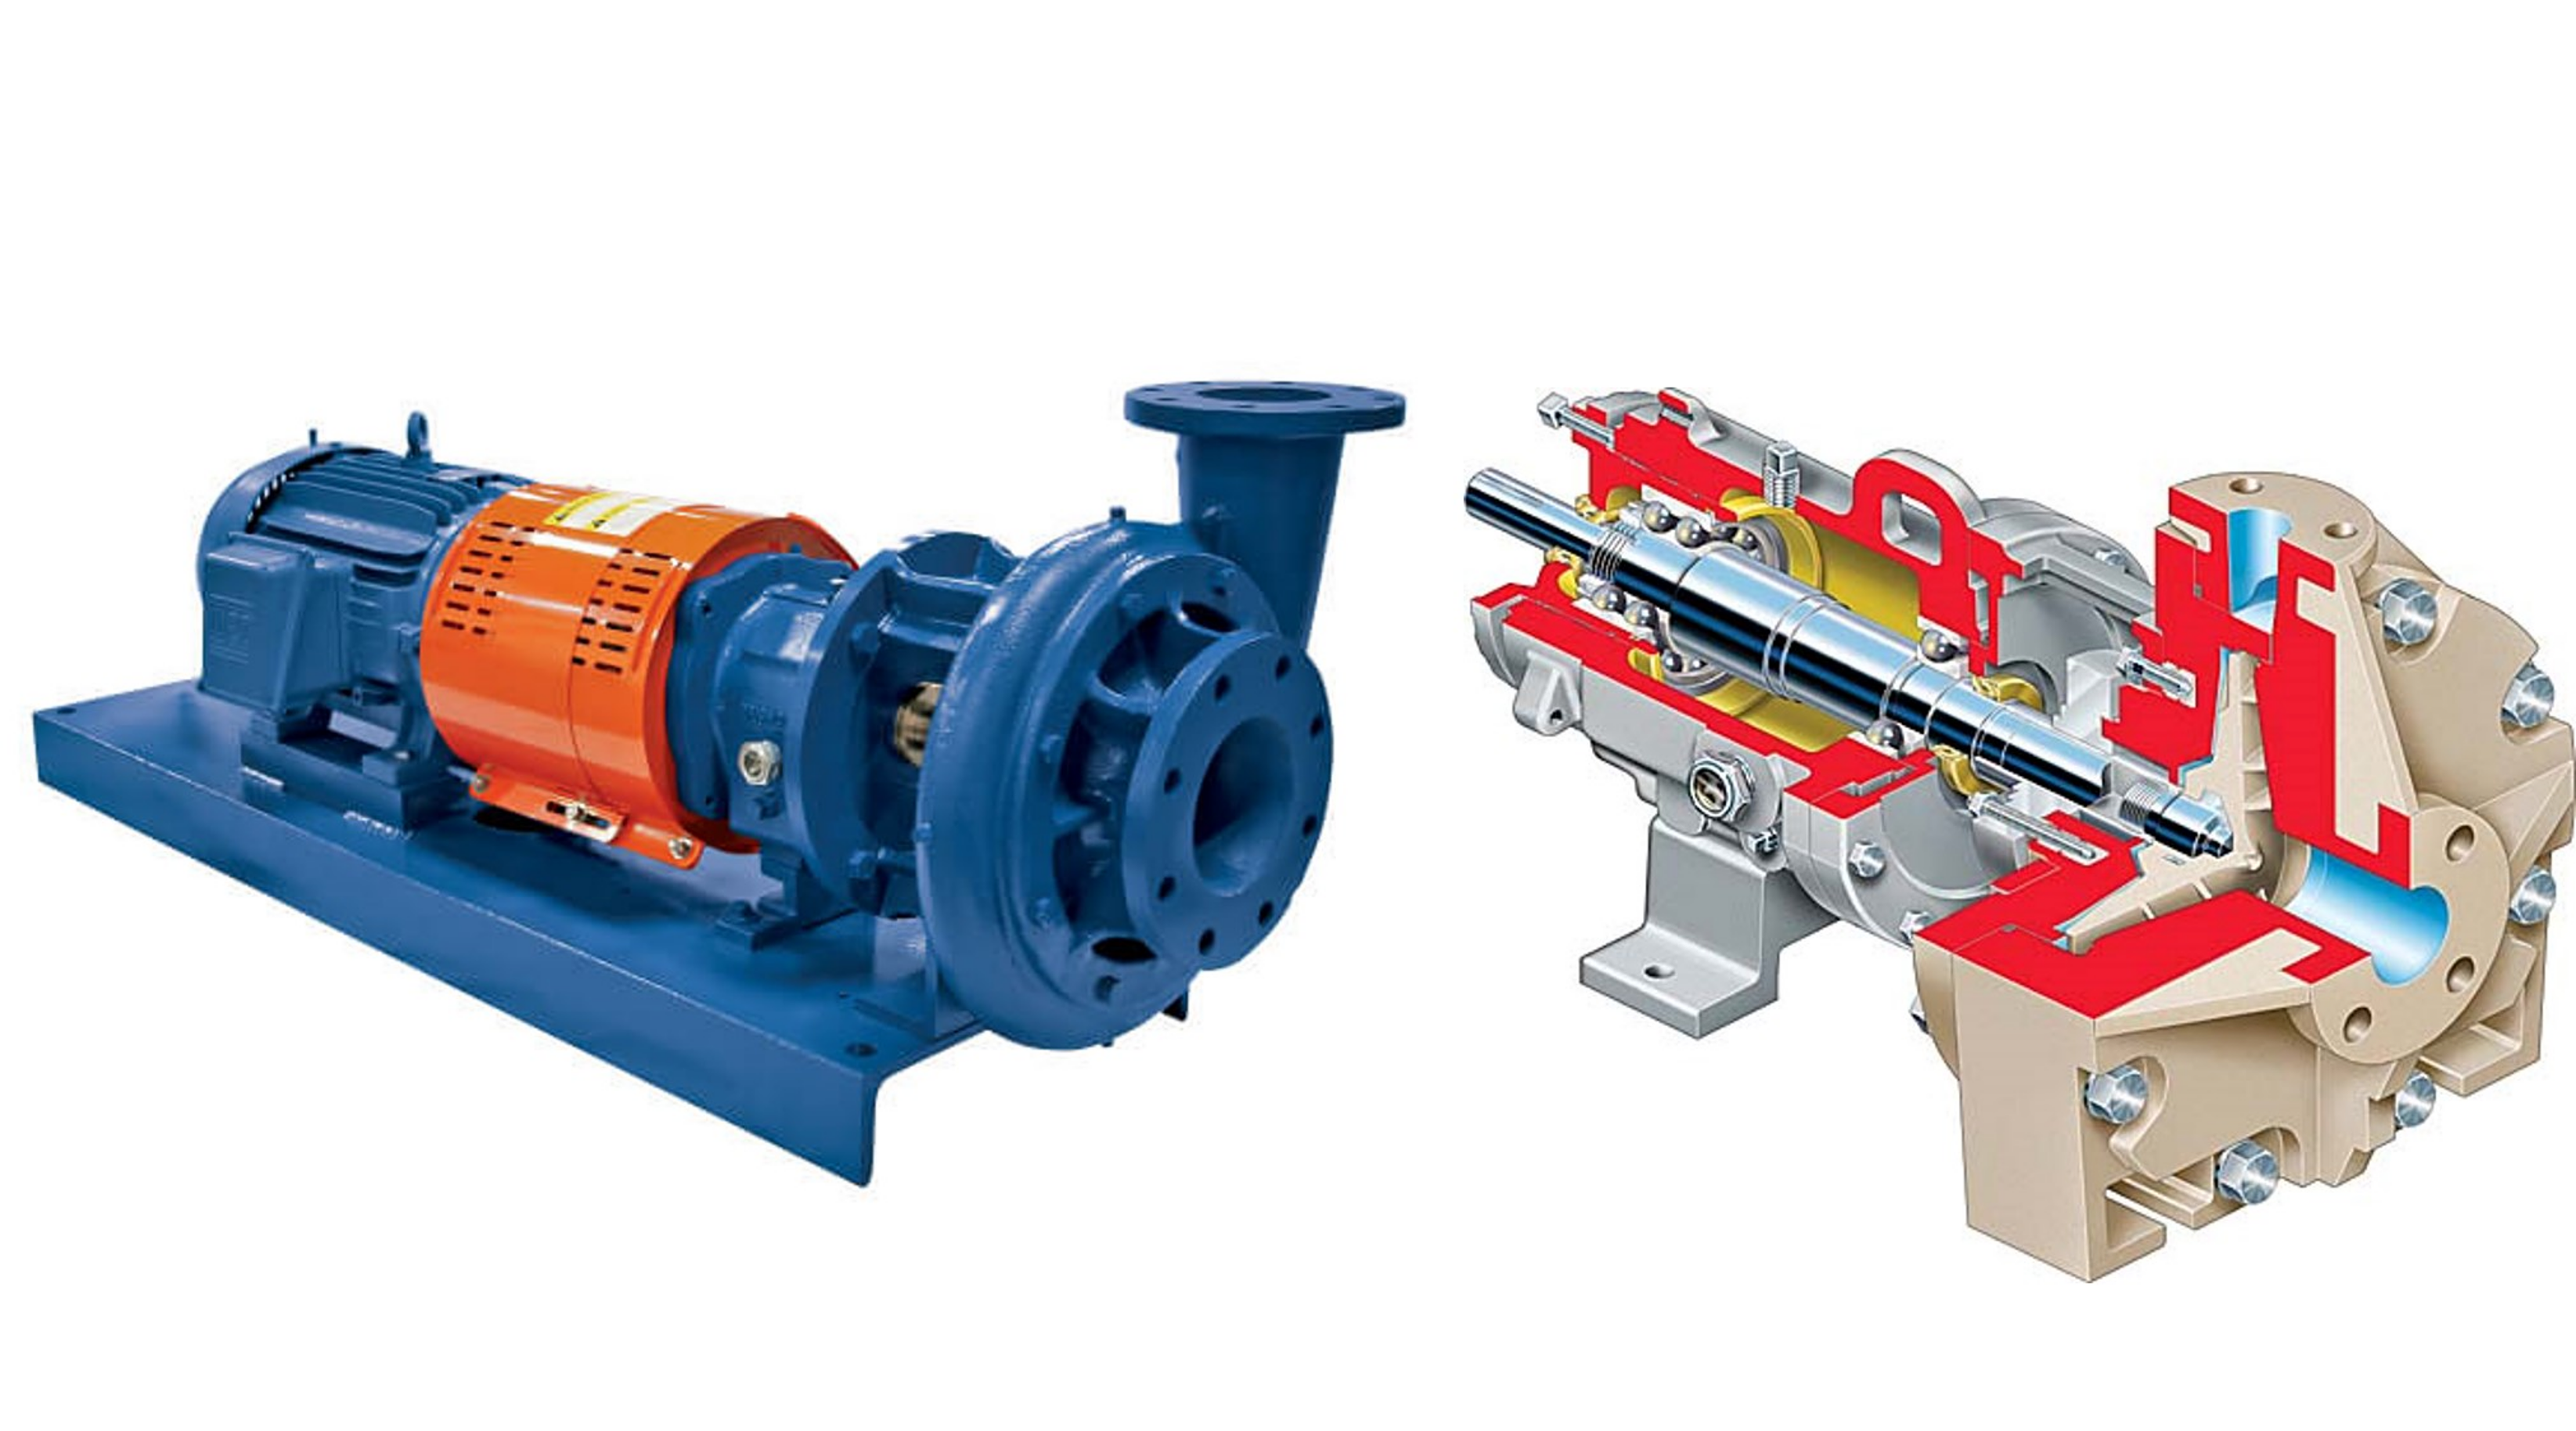
\includegraphics[scale=0.6]{FrameMounted}
%\caption{Frame mounted end-suction pump}
%\end{center}
%\end{figure}
\item Close-coupled:  A close-coupled pump has only one shaft and one set of bearings: the motor shaft and bearings. The pump impeller is placed directly onto the motor shaft. Close-coupled pumps require less space and are less expensive than frame-mounted pumps.


\begin{figure}[h!]
\begin{tabular}{  m {8cm}  m {8cm} } 
\begin{center}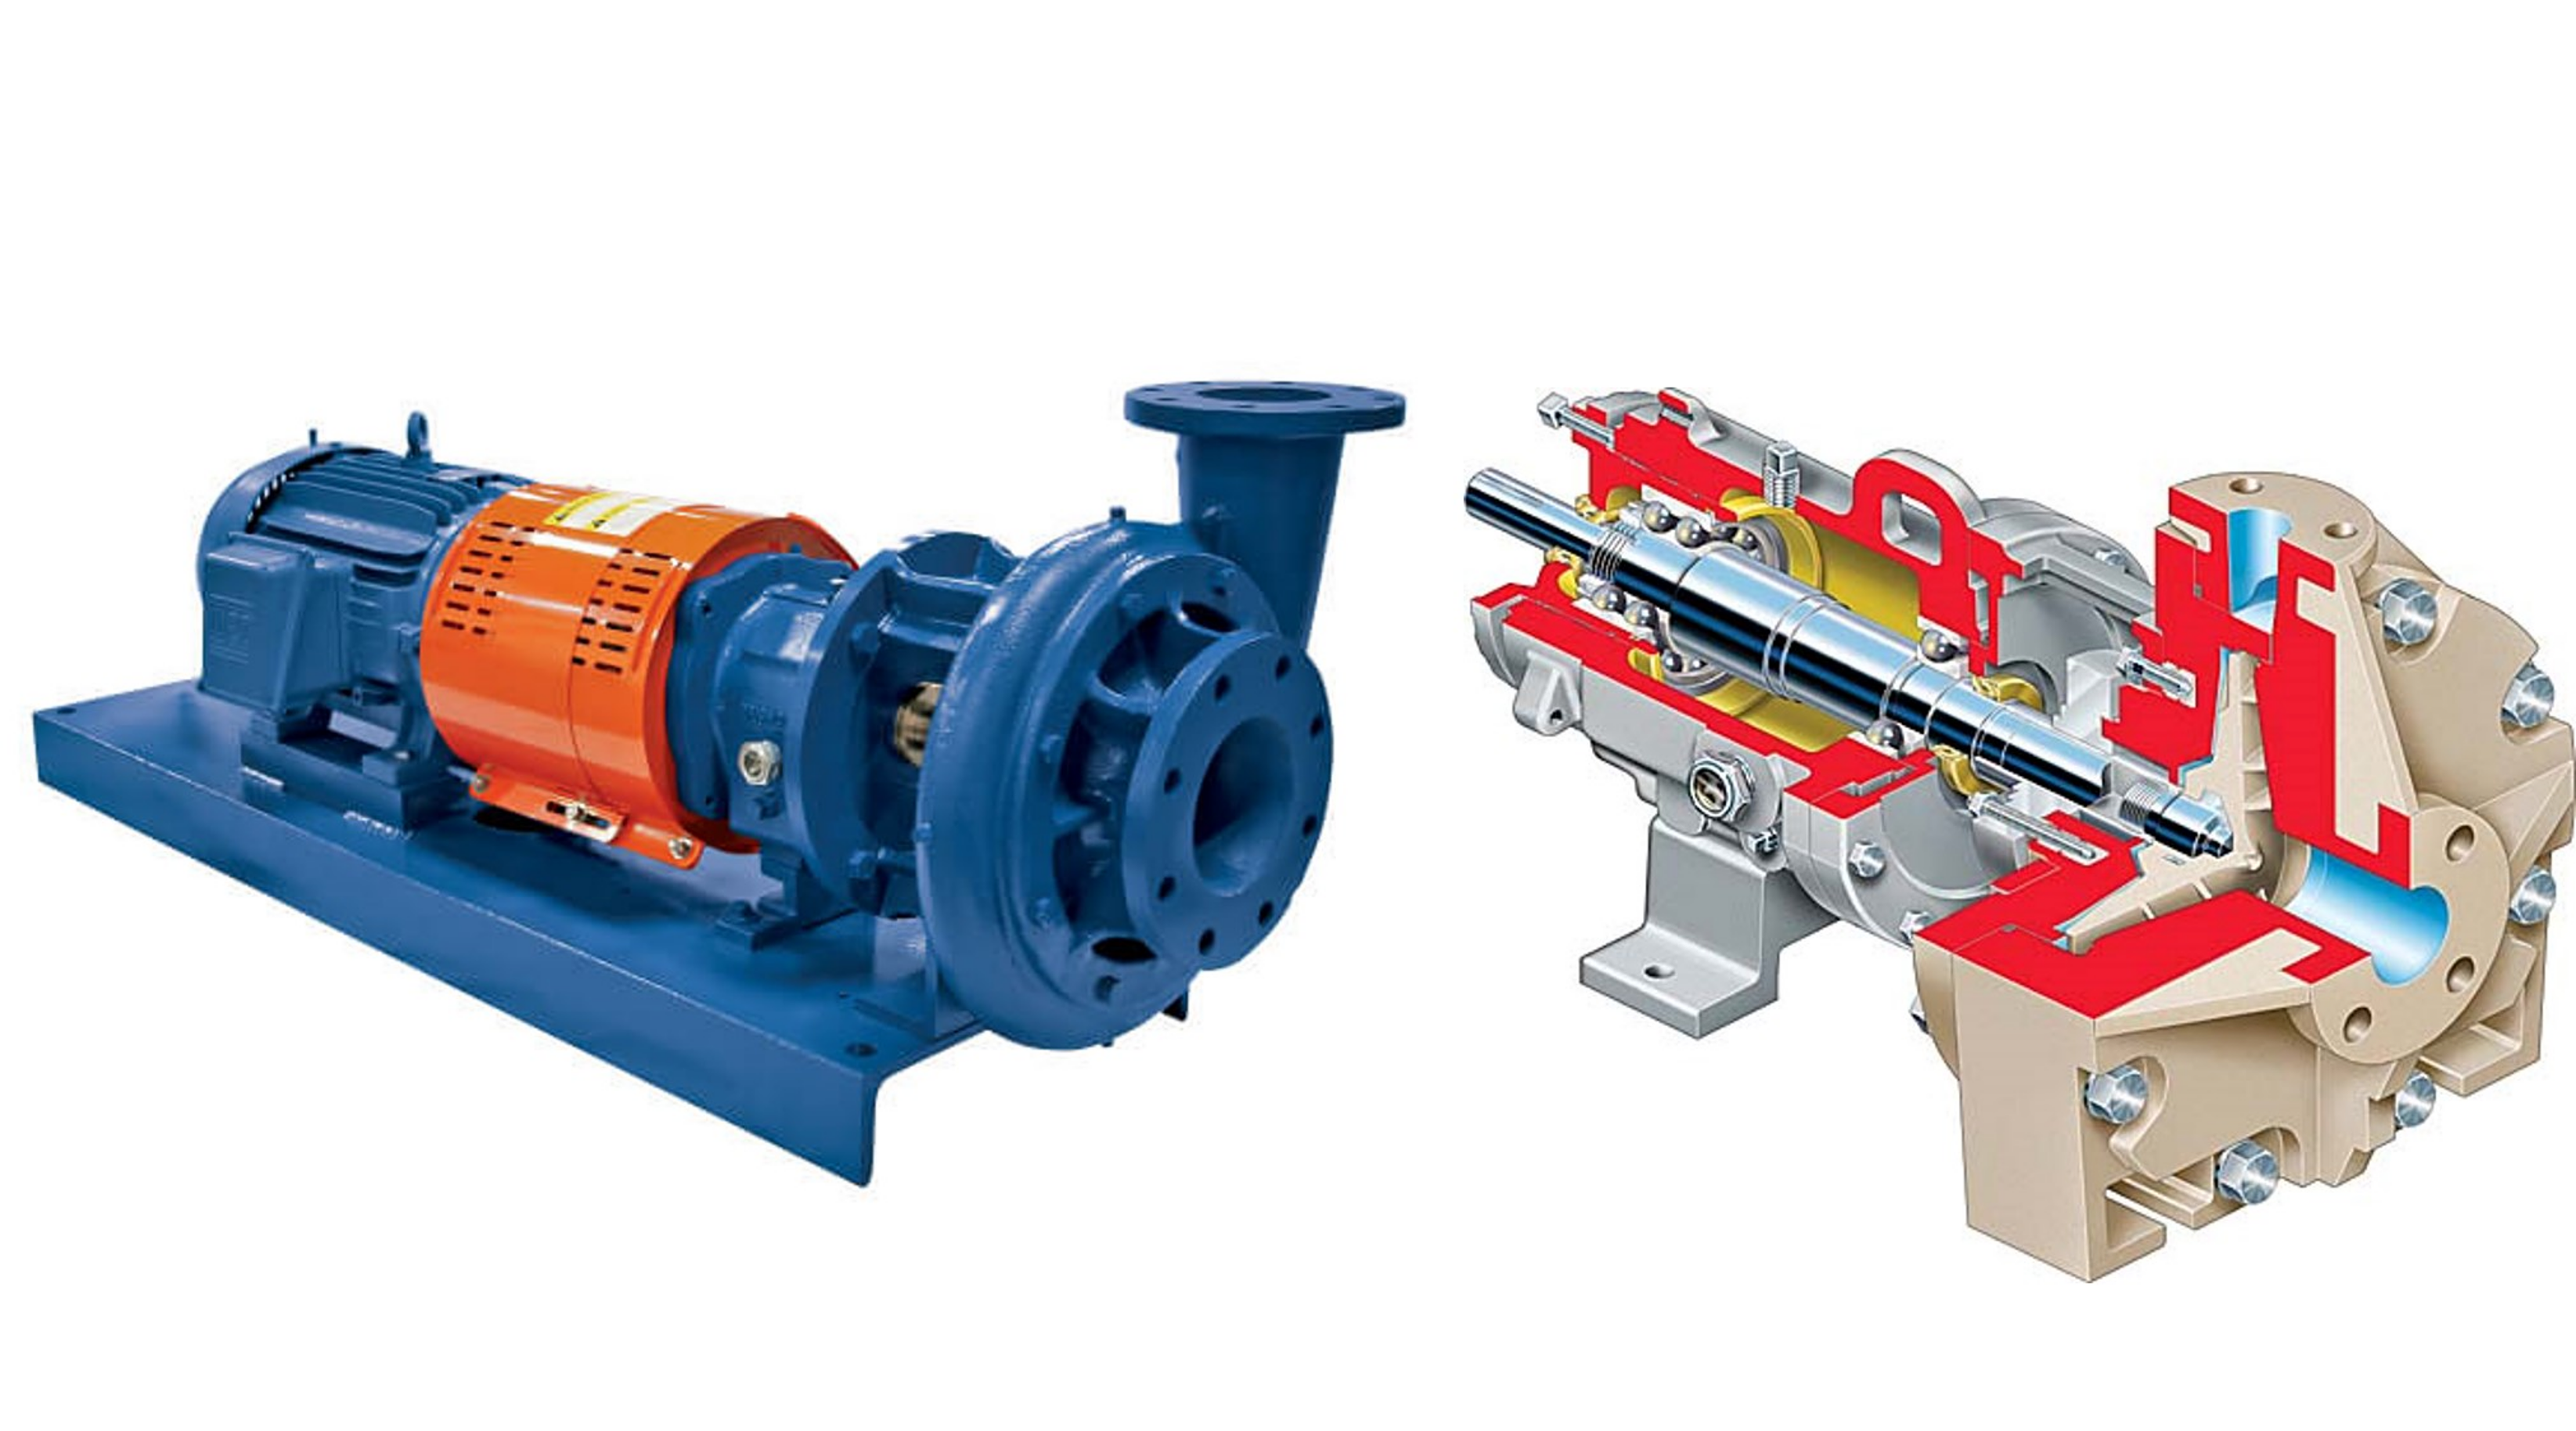
\includegraphics[scale=0.27]{FrameMounted} \end{center} & \begin{center} \includegraphics[scale=0.4]{CentrifugalCloseCoupledPump} \end{center}\\
\begin{center} \textbf{Frame Mounted End-Suction Pump} \end{center} & \begin{center}\textbf{Close-Coupled Pump} \end{center}\\
\end{tabular}\\
\end{figure}



%\begin{figure}[h!]
%\begin{center}
%\includegraphics[scale=0.8]{CloseCoupledPump}
%\caption{Close-coupled end-suction pump}
%\end{center}
%\end{figure}
\end{itemize}
\item Split-case centrifugal pumps\index{Centrifugal pumps!Split case}:
\begin{itemize}
\item A centrifugal pump designed so that the volute case is split horizontally.
\item The case divides on a plane that cuts though the eye of the impeller.
\item This design allows easy access to the pump’s internal parts for maintenance.  
\item Split-case pumps are used in high flow applications including water treatment plants for distributing potable water and for fire protection.  
\item Split-case pumps are classied based upon their case design:
\begin{itemize}
\item Radial Split – Radially split pump casing opens perpendicular to the shaft axis and parallel to the impeller.     

\item Axial Split – In this design, the pump casing is spliced into two halves that get separated horizontally, or you can say that parallel to the shaft axis.
\end{itemize} 
\begin{figure}[h!]
\begin{center}
\includegraphics[scale=0.21]{CentrifugalSplitCasePumpRadialAxial}
\caption{Horizontal Split-case pumps Radial and Axial }
\end{center}
\end{figure}
\end{itemize}
\end{itemize}
\end{enumerate}
\newpage
\subsection{Axial-flow pumps}\index{Pump type!Axial-flow pumps}
\begin{figure}[h!]
\begin{center}
\includegraphics[scale=0.08]{AxialFlowPump}
\caption{Axial flow pump}
\end{center}
\end{figure}
\begin{itemize}
\item Utilizes a propeller driven by a sealed motor in a pipe to impart the hydraulic energy.  \item Unlike the centrifugal pumps, the direction of flow is unchanged in axial-flow pumps.
\item The axial flow 
\item Axial flow pumps are characterized by the highest flow rates and lowest discharge pressures.  
Vertical turbine pump - These type of centrifugal pumps are primarily mounted with a  vertical shaft; the motor is commonly mounted above the pump. Vertical turbine pumps are either mixed or axial flow devices.  

\end{itemize}

\subsection{Mixed-flow pumps}\index{Pump type!Mixed-flow pumps}
\begin{itemize}
\item Mixed flow pumps borrow design characteristics from both axial and radial pumps. 
\item Their design includes a diagonally operating impeller that uses centrifugal force to direct the water out of the pump and give it an axial pushing action. 
\item This dual pumping action enables mixed flow pumps to have higher mass flow rate of axial pumps with higher pressure of centrifugal pumps.
\item Therefore, mixed flow pumps are ideal for any application that requires the pumps to operate within the gap left between axial and radial pumps.
\end{itemize}
\section{Positive displacement pump}\index{Pump type!Positive displacement pumps}
\begin{itemize}
\item A positive displacement pump operate by forcing a fixed volume of fluid from inlet pressure section of the pump into the discharge zone of the pump. 
\item Positive displacement pumps are a category of pumps designed to move fluid at a steady rate through a system.
\item These pumps are able to handle viscous fluids, which flow at lower speeds and create more resistance, more efficiently than kinetic (dynamic) pumps.
\item These pumps cannot achieve high flow rates and are typically used not for pumping water.
\item They are used typically for chemical dosing applications including dosing coagulants and flocculants as they are more efficient in applications involving low flows of higher viscosity fluid.
\item Displacement pumps will not change their volume with a change in discharge pressure.
\item It can be classified into two types:
\begin{enumerate}
\item Rotary-type positive displacement pump: 
\begin{itemize}
\item This pump can move the fluid by using a rotating mechanism that creates a vacuum that captures and draws in the liquid. 
\item Rotary positive displacement pump can be classified into two main types:
\begin{itemize}
\item Gear Pump:
\begin{figure}[h]
\begin{center}
\includegraphics[scale=0.4]{GearPumps}
\caption{Gear Pumps}
\end{center}
\end{figure} 
\begin{itemize}
\item This pump provides a constant volume of fluid that passes between the teeth of two meshing gears and the casing.
\item The rotating gears and separation of teeth create a suction that pulls fluid in through the inlet. 
\item The gears then trap the liquid and move it around the casing to the discharge or outlet. \item Each revolution creates consistency in the flow of fluid.
\item There are two main types of rotary gear pumps - internal and external which are differentiated by the way the gear teeth lock together.
\end{itemize}
\item Lobe pump: 
\begin{figure}[h]
\begin{center}
\includegraphics[scale=0.55]{LobePump1}
\caption{Lobe Pump}
\end{center}
\end{figure}
\begin{itemize}
\item Lobe pumps are like gear pumps in that fluid flows around the interior of the casing, but they use lobes instead of the gears with teeth. 
\item The lobes do not touch each other, thus reducing wear, and they are driven by external timing gear which can allow the lobe pump to operate in either direction.
\item Rotary lobe pumps are capable of handling thick fluids that are laden with solids. Their gentle handling of solids works well mixed with low viscosity substances.
\end{itemize}
\item Screw pump: 
\begin{figure}[h]
\begin{center}
\includegraphics[scale=0.25]{ScrewPump}
\caption{Screw pump - Twin-screw type}
\end{center}
\end{figure}
\begin{itemize}
\item Screw pumps and twin-screw pumps use rotating screws to move liquids and solids from one end of the pump to the other. 
\item The turning action creates a spinning motion that pumps material. 
\item The twin-screw pumps are identical to the screw pump, but with a dual screw for more power. \item Screw pumps are capable of high flow rates with very little to no vibration.
\end{itemize}
\end{itemize}
\end{itemize}
\item Reciprocating-type positive displacement pump: 
\begin{itemize}
\item This pump works by the repeated back-and-forth movement (strokes) of either a piston, plunger or diaphragm. 
\item Types of this pump are:
\begin{itemize}
\item Piston pump:  In a piston pump, the first stroke of the piston creates a vacuum, opens an inlet valve, closes the outlet valve and draws fluid into the piston chamber (the suction phase). As the motion of the piston reverses, the inlet valve, now under pressure, is closed and the outlet valve opens allowing the fluid contained in the piston chamber to be discharged (the compression phase). 
\item Plunger pump:  The plunger pump works similar to the piston pump.  The volume of fluid moved by a piston pump depends on the cylinder volume; in a plunger pump it depends on the plunger size. 
\item Diaphragm Pump: A diaphragm pump uses a flexible membrane instead of a piston or plunger to move fluid. By expanding the diaphragm, the volume of the pumping chamber is increased and fluid is drawn into the pump. Compressing the diaphragm decreases the volume and expels some fluid. Diaphragm pumps have the advantage of being hermetically sealed systems making them ideal for pumping hazardous fluids.
\end{itemize}
\begin{figure}[h!]
\begin{center}
\includegraphics[scale=0.6]{ReciprocatingPumpsDesign}
\caption{Reciprocating Pumps Design}
\end{center}
\end{figure}
%
%\begin{center}
%\includegraphics[scale=0.25]{DoubleDiaphragmPump}\\
%\caption{Diaphragm pump - Double diaphragm type}
%\end{center}

\item The cyclic action of reciprocating pumps creates pulses in the discharge with the fluid accelerating during compression and slowing down during the suction phase.
\item Pulsing can be minimized by using two or more pistons, plungers or diaphragms with on in its compression phase whilst the other is in suction.
\item The repeatable and predictable action of reciprocating pumps make them ideal for applications where accurate metering or dosing is required.
\end{itemize}
\end{enumerate}
\end{itemize}

\section{Turbine pumps}\index{Pump type!Turbine pumps}
\begin{itemize}

\item Turbine pumps are centrifugal in nature but have some characteristics of positive displacement. 

\item First, the way they impart energy to the liquid is kinetic (and hence centrifugal) in nature. However, they typically have multiple “stages,” with each stage generating a little incremental pressure. Since each stage is incremental, the risk of cavitation is lower.

\item Clearances are said to be very tight, and hence, the reference to them having some characteristics of positive displacement pumps.

\item They are often used in high head but relatively low-volume applications, such as pumping water a significant height.  Typical applications include wells that are bored to provide agricultural or turf irrigation, or to provide water supply for municipalities that rely on ground water rather than surface water. They are also used to provide plant make-up water and fire water for industrial plants.

\item Mostly due to their compact size and multiple stage capability, their typical application is with clean water (fresh or waste) with minimal solids content. (Their relatively close tolerances cannot long survive abrasive slurries such as drilling muds.)

\item The term “turbine” in the pump name is somewhat of a misnomer, as this pump type has nothing to do with a turbine.

\item The pump end consists of at least one rotating impeller that is attached to a shaft and directs the well water into a diffuser casing called a bowl.

\item This pump is often staged – that is, designed with more than one impeller. Each additional impeller increases the amount of head the pump can produce while the flow remains unchanged.

\item In a staged turbine pump, water enters the pump at the bottom through a bell-shaped part called the suction bell. From there it moves into the first stage impeller, which raises the water’s velocity. The water then enters the diffuser bowl immediately above the impeller, where this high velocity energy is converted into high pressure. The bowl also directs the fluid into the next impeller located immediately above the bowl, and this process continues through all of the stages of the pump. 

\item The two main types of turbine pumps are vertical turbine pumps and submersible turbine pumps.

\item While submersible pumps have the electric motor located underwater at the bottom of the pump, vertical turbine pumps have the motor located above ground, connected via a long vertical shaft to impellers at the bottom of the pump. 

\begin{figure}[h!]
\begin{center}
\includegraphics[scale=0.3]{TurbinePumps}
\caption{Turbine Pumps}
\end{center}
\end{figure}

\end{itemize}

\section{Choosing between positive displacement and centrifugal pumps}\index{Pumps!Choosing between positive displacement and centrifugal pumps}
\begin{itemize}
\item Common Positive Displacement Pump Applications and Handled Fluids:
\begin{itemize}
\item High-viscosity fluids (e.g., chemicals including polymers)
\item High-pressure requirements
\item Low flow rate requirements
\end{itemize}
\item Common Centrifugal Pump Applications and Handled Fluids:
\begin{itemize}
\item Most water pumping applications
\item High-flow applications
\end{itemize}
\end{itemize}

\section{Components of centrifugal pumps}\index{Centrifugal Pumps!Components}


\begin{figure}[h!]
\begin{center}
\includegraphics[scale=0.25]{CentrifugalPumpComponents1}
\caption{Centrifugal Pump Components}\index{Pumps!Centrifugal pump components}
\end{center}
\end{figure}

The mechanical parts of a typical rotodynamic pump include:
\begin{itemize}

\item Wear Rings:\index{Centrifugal Pumps!Components!Wear rings}\\
With closed impellers, the impeller fits very close to the case. As a result, the case is worn by material passing from the high-pressure side to the low-pressure side of the impeller. To protect the case, brass or stainless steel wear rings are inserted into the case which creates the contact area between rotating and stationary parts inside the pump.

\item Volute Case:\index{Centrifugal Pumps!Components!Volute case}\\
Around the impeller is the volute case. The volute case gathers the water thrown from the impeller and directs it in a single direction.

\item Backing Plate:\index{Centrifugal pump components!Backing plate}\\
Behind the volute case is the backing plate. The backing plate seals the back of the volute case area.

\item Stuffing Box:\index{Centrifugal Pumps!Components!Stuffing box}\\
The stuffing box is located at the back of the impeller and around the shaft.   It is attached to, and sometimes part of, the backing plate.  It houses the packing or mechanical seal and is usually referred to as the dry portion of the pump.

\item Shaft:  \index{Centrifugal Pumps!Components!Shaft}\\
The impeller is attached to a shaft. The shaft is often made of steel or stainless steel to support the impeller. The sizes of the shafts must be measured accurately. An undersized shaft may increase pump vibration, reduce bearing life, cause shaft breakage, and shorten the overall pump life. On the other hand, an oversized shaft can unnecessarily increase the pump costs.

\item Shaft Sleeve: \index{Centrifugal Pumps!Components!Shaft sleeve}\\
Usually, a portion of the shaft located below the seals is covered with a shaft sleeve. The shaft sleeve is made of a metal, generally bronze or stainless steel. It is designed to operate with the ability to slide or thread on the shaft. The shaft sleeve is applied to properly position the impeller on the shaft as well as to protect the shaft.

\begin{figure}[hbt!]
\begin{center}
\includegraphics[scale=0.13]{CentrifugalPumpShasftSleeveThreadedtoShaft}
\caption{Shaft sleeve threaded to shaft}
\end{center}
\end{figure}

\item Seals:\\
\begin{itemize}
\item The place where the shaft passes through the casing is the stuffing box must be sealed to prevent the pressurized water from the "wet" end of the pump to escape the rotating shaft in the stuffing box.

\item Typically either a mechanical seal or a packing seal (traditional method) are used for stopping this leakage. 

\item Packing/Mechanical Seals:\index{Centrifugal Pumps!Components!Packing/mechanical seals}\\
Packing and mechanical seals serve the same purpose: they control leakage through the stuffing box. 

\begin{itemize} 
\item Packing:  A packing is composed of some type of fiber, like cotton, and some type of lubricant, like graphite or Teflon. Packing seals are rings of braided, fibrous material.  are housed in a are “stuffed” into a pump stuffing box (or seal chamber), located around the outside diameter of the pump shaft, to reduce the amount of pumped medium that is forced out of the pump along the drive shaft.
\item Mechanical seal:  A mechanical seal is composed of two finely machined surfaces, one hard and one soft, that prevent water from passing. When installing packing, joints should be staggered.
\end{itemize}


%\begin{figure}[h!]
%\begin{tabular}{  m {5cm}  m {5cm} m{5cm}} 
%\begin{center} \includegraphics[scale=0.3]{CentrifugalPumpOperatingPrinciple} \end{center} & \begin{center}\includegraphics[scale=0.25]{CentrifugalPumpCase} \end{center} & \begin{center}\includegraphics[scale=0.18]{CentrifugalPumpStuffingBox} \end{center}\\
%\begin{center} \textbf{Operating Principle} \end{center} & \begin{center}\textbf{Pump Casing} \end{center}  & \begin{center}\textbf{Stuffing Box} \end{center}\\
%\end{tabular}\\
%\end{figure}

\begin{figure}[h!]
\begin{tabular}{  m {5cm}  m {5cm} m{5cm}} 
\begin{center}\includegraphics[scale=0.25]{CentrifugalPumpStuffingBox1} \end{center} & \begin{center} 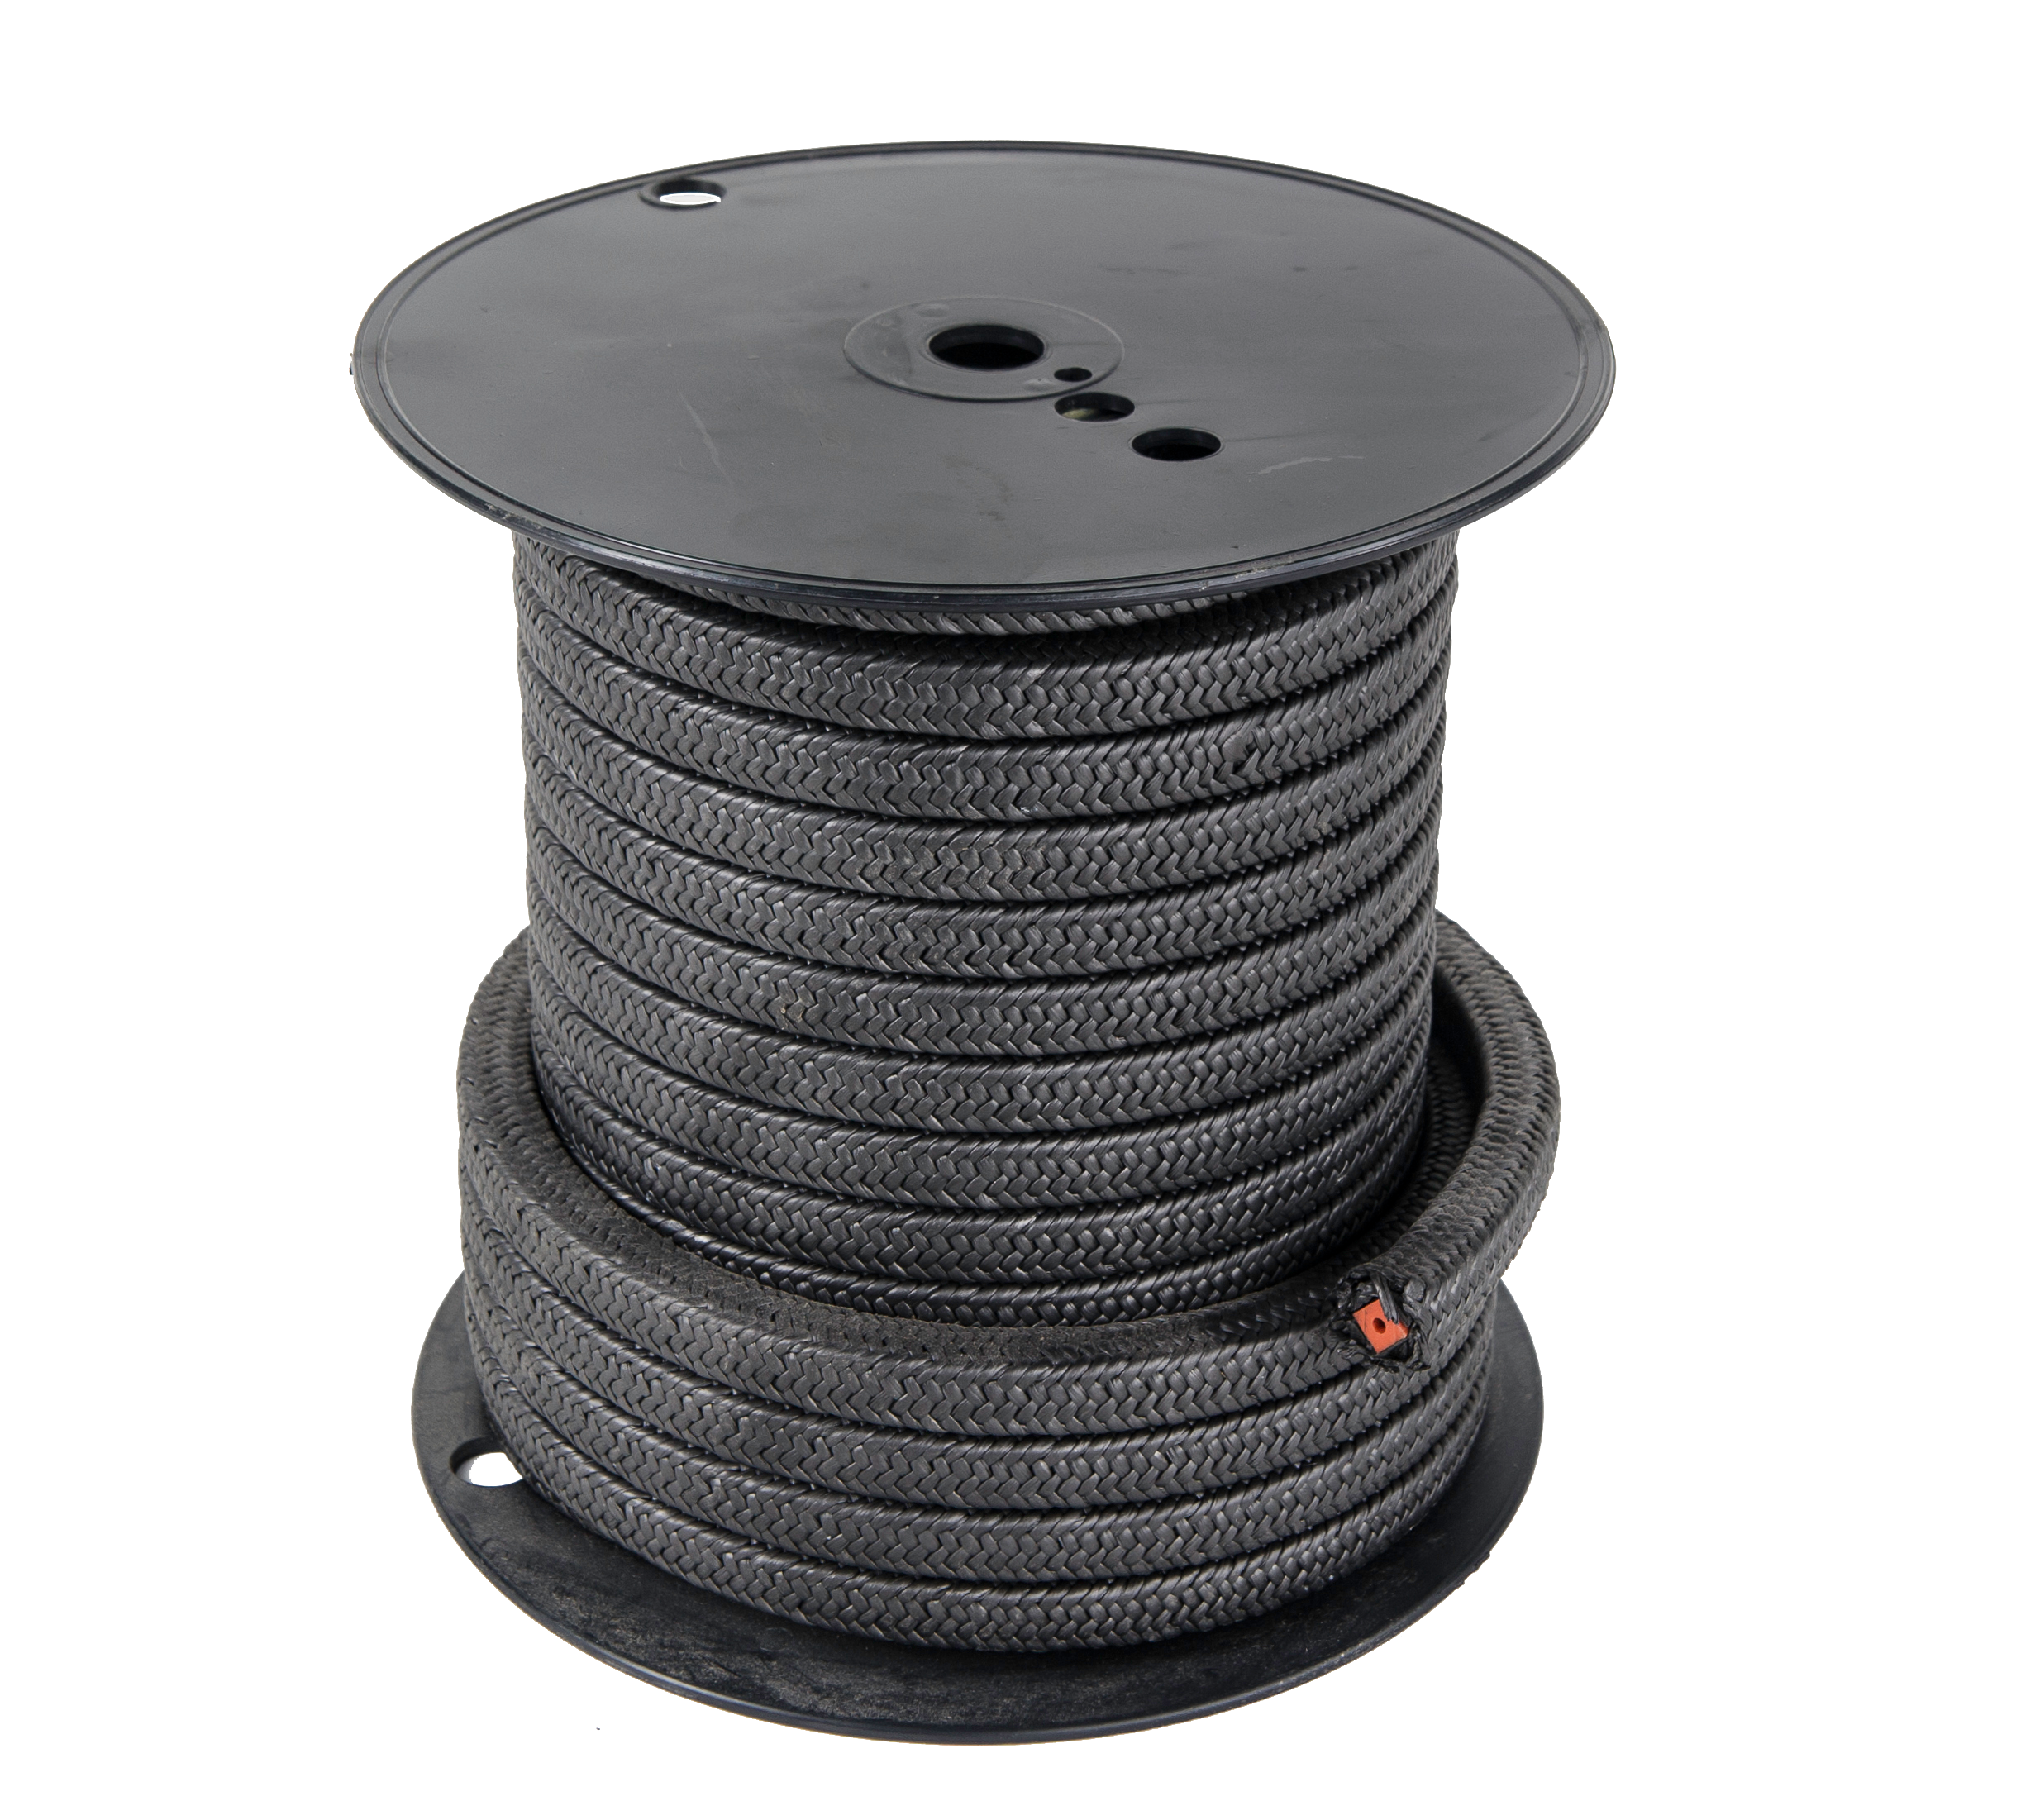
\includegraphics[scale=0.05]{CentrifugalPumpBraidedPacking1} \end{center} & \begin{center}\includegraphics[scale=0.12]{CentrifugalPumpMechanicalSeal} \end{center}\\
\begin{center} \textbf{Stuffing Box} \end{center} & \begin{center}\textbf{ Braided Packing} \end{center}  & \begin{center}\textbf{Mechanical Seal} \end{center}\\
\end{tabular}\\
\end{figure}
\end{itemize}
\item Packing Gland:\index{Centrifugal Pumps!Components!Packing gland}\\
In order to control leakage with packing, pressure must be placed on the packing. This pressure is applied by the packing gland, two pieces of metal at the back of the stuffing box. There should be a slow drip from the stuffing box to show lubrication between the shaft and the packing.

\item Lantern Ring:\index{Centrifugal Pumps!Components!Lantern ring}\\
It is often desirable to lubricate and cool the packing with external water or oil. When water is used, it is called seal water or flush water. The seal water is distributed into the stuffing box through the lantern ring, which is commonly a brass ring with holes that allow the water to easily pass.

\item Gland: \index{Centrifugal Pumps!Components!Gland}The gland is located around the shaft of the pump and bolts to the face of the stuffing box directly on the pump casing.  The gland nut allows the packing material to be compressed to form a watertight seal and prevent leakage of the pumped water.

\item Both, packing seals and mechanical seals, rely on seal water for effective operation. Seal water serves three main purposes: to cool the seal and the shaft, to lubricate the seal and to flush away impurities in the system.

\end{itemize}


\section{Pump maintenance} \index{Pump maintenance}
\begin{itemize}
\item Maintenance strategies can be generally classified as:
\begin{enumerate}
\item Corrective maintenance: 
\begin{itemize}
\item Corrective maintenance is maintenance that is undertaken in response to the equipment failure.
\item It is a reactive maintenance activity and is not focused on prolonging asset life and its practice results in largest pumping system downtime.
\end{itemize}
\item Preventative maintenance:
\begin{itemize}
\item It involves planned and scheduled maintenance activities to help prevent unexpected failures of the equipment. 
\item It also involves predictive maintenance which utilize equipment monitoring over time to monitor the equipment condition.
\item Preventive maintenance tends to extend the lifespan of assets.
\end{itemize}
\end{enumerate}
\item Preventative pump maintenance:\\
\begin{itemize}
\item A pump maintenance program would generally involve a periodic check of the pump performance, an inspection of the wearing parts and lubrication of bearings and joints. 
\item It is good practice to carry out a visual inspection of the pump installation on a daily basis. Spotting an issue early is one of the best methods of trouble shooting and preventing pump breakdown.
\item Most of the things to look out for should be easily visible, these include:
\begin{itemize}
\item Pump seals:
\begin{itemize}
\item Mechanical seals are a wearing part and need to be routinely replaced.
\item Pump packing must be inspected regularly to ensure a steady leak rate of about 10-15 drops per minute.
\item Packing must be monitored daily and may be adjusted as needed to maintain this rate and replaced when it becomes worn or damaged.  
\item The leakage cools and lubricates the packing.  Without leakage, the packing will burn and wear grooves into the shaft and sleeves.
\item When installing new packing, stagger the joints of each packing ring 90 degrees, beginning at twelve o’clock, three o’clock, six o’clock, and then nine o’clock.
\end{itemize}
\item Unusual noise:
\begin{itemize}
\item While a consistent hum when the pump is running is quite normal, abnormal loud noises or a clunking or crunching sound is likely to indicate an issue e.g. worn bearings.
\item A popping sound, particularly if it is near the impeller, could mean the pump is experiencing cavitation which can cause a lot of damage.
\end{itemize}
\item Extreme vibration: A properly installed, well working pump should not overly vibrate, and therefore any level of vibration deemed excessive should be investigated. Common causes include impeller imbalance, damage and misalignment of the pump and motor.
\item Overheating: The pump, motor or bearings getting really hot is not something that should be ignored as it always indicates some form of problem which may include - internal rubbing/wearing of parts, that the wrong power has been put into the pump, the pump has been running against a dead head or that it has been running at a duty it cannot efficiently maintain.
\item Lubrication: Lubricate the motor and pump bearing per manufacturer's guidelines. Be sure not to over lubricate. More bearing damage occurs as a result of over greasing than under greasing.
\item Pump motor meggar testing:
\begin{itemize}
\item Meggar testing assesses the integrity of electrical insulation in the motor.
\item Low resistance is caused by the degradation of the insulation of the windings due to conditions such as overheating, corrosion, or physical damage.
\item Degraded insulation inside the motor leads to insufficient isolation between the conductors or motor windings, which can cause leakages and short circuits, and eventually motor failure.
\item Megger testing involves applying a high-voltage DC potential to the motor's insulation system and measuring the resulting current flow.  
\item It is always good to conduct motor testing at least once every six months.
\end{itemize}
\end{itemize}
\end{itemize}
\end{itemize}

\section{Pump calculations}\index{Pumping!Pump calculations}
\begin{itemize}
\item Pump is a machine used for moving water (and other fluids) through a piping system and raise the pressure of the water.
\item Pumping is accomplished by transforming the input energy - typically from an electric motor or from other sources such as high-pressure air.
\item The pump calculations in this section are for electrically driven rotodynamic pumps.
\item To move water, a pump will need to overcome resistance due its density, gravitational force and friction.
\item This resistance is dependent on:
\begin{itemize}
\item Height the water needs to be raised.  This height of the fluid in a container is referred to as head. 
\item Quantity of water involved
\end{itemize}
\end{itemize}

\subsection{Glossary of pump calculations terms}\index{Pumping!Glossary of pump calculations terms}

\textbf{Force:} \index{Pumping!Force} In the English system force and weight are often used in the same way. The weight of the cubic foot of water is $62.4$ pounds. The force exerted on the bottom of the one foot cube is $62.4$ pounds. If we have two cubes stacked on top of one another, the force on the bottom will be $124.8$ pounds.

\textbf{Pressure:} \index{Pumping!Pressure} Pressure is a force per unit of area, pounds per square inch or pounds per square foot are common expressions of pressure. The pressure on the bottom of our cube is $62.4$ pounds per square foot. It is normal to express pressure in pounds per square inch (psi). This can be accomplished by determining the weight of one square inch of our cube one foot high. Since the cube is 12 inches on each side, the number of square inches on the bottom surface of the cube is $12 \times 12=144 \mathrm{in}^{2}$. Now by dividing the weight by the number of square inches we can determine the weight on each square inch.

\textbf{Head:}  \index{Pumping!Head}Pressure is directly related to the height of a column of fluid. This height is called head or feet of head. Pressure and feet of head head are directly related - \emph{for every one foot of head there is a pressure of $0.433$ psi.}

\vspace{0.2cm}
Thus, $\dfrac{0.433 \enspace psi}{ft \enspace (water \enspace column)}$ or conversely $\dfrac{1 \enspace ft \enspace (water \enspace column)}{2.31 \enspace psi}$\\
\vspace{0.2cm}
\textbf{Note:  This pressure/head will include the height the water pumped and also the head associated with friction losses - energy loss because of the water moving through the pipe and fittings.}\\

\begin{figure}[h]
\begin{tikzpicture}
\path[help lines,step=.2] (0,0) grid (16,6);
\path[help lines,line width=.6pt,step=1] (0,0) grid (16,6);
%\foreach \x in {0,1,2,3,4,5,6,7,8,9,10,11,12,13,14,15,16}
%\node[anchor=north] at (\x,0) {\x};
%\foreach \y in {0,1,2,3,4,5,6}
%\node[anchor=east] at (0,\y) {\y};
\pgfmathsetmacro{\cubex}{3}
\pgfmathsetmacro{\cubey}{3}
\pgfmathsetmacro{\cubez}{3}
\draw(13.5,5,3) -- ++(-\cubex,0,0) -- ++(0,-\cubey,0) -- ++(\cubex,0,0) -- cycle;
\draw(13.5,5,3) -- ++(0,0,-\cubez) -- ++(0,-\cubey,0) -- ++(0,0,\cubez) -- cycle;
\draw(13.5,5,3) -- ++(-\cubex,0,0) -- ++(0,0,-\cubez) -- ++(\cubex,0,0) -- cycle;
\draw (8.7,2.5) node[text width=3cm,align=center]
  {\scriptsize{12"}};
\draw (14.1,3.4) node[text width=3cm,align=center]
  {\scriptsize{12"}};
  \draw (10.9,0.5)node[text width=3cm,align=center]
  {\scriptsize{12"}};
    \draw (2.8,4.8)node[text width=3.8cm,align=left]
  {\small{$Pressure=\dfrac{Force}{Area}$}};
      \draw (2.8,3.1)node[text width=3.8cm,align=left]
  {\small{Pressure exerted by}};
        \draw (2.8,2.8)node[text width=3.8cm,align=left]
  {\small{a 1ft column of water}};
        \draw (5.3,2.9)node[text width=3cm,align=center]
  {\small{$=\dfrac{62.4 \enspace lb}{12 in \enspace x \enspace 12 in}$}};
          \draw (7.3,2.9)node[text width=3cm,align=center]
  {\small{$=0.43 \enspace psi$}};
         \draw (3.45,1.2)node[text width=5cm,align=left]
  {\small{As 1$ft^3$ of water weighs 62.4 lbs}};
\end{tikzpicture}
\end{figure}


The pressure at the bottom of a container is affected only by the height of water in the container and not by the shape or the volume of the container. In the drawing below there are four containers all of different shapes and sizes. The pressure at the bottom of each is the same.

\begin{center}
\includegraphics[scale=0.2]{2022_11_03_65aa625ded296bdfd01fg-17}
\end{center}
The pressure exerted at the bottom of a tank is relative only to the head on the tank and not the volume of water in the tank. For example, below are two tanks each containing 5000 gallons. The pressure at the bottom of each is 22 psi. If half of the water were drained from the tanks the pressure at the bottom of the elevated tank would be $17.3$ psi while the pressure at the bottom of the standpipe would be 11 psi.\\

\begin{center}
\includegraphics[scale=0.25]{2022_11_03_65aa625ded296bdfd01fg-18}
\end{center}

\textbf{Velocity: } \index{Pumping!Velocity} Velocity is the speed that the water is moving along a pipe or through a basin. Velocity is usually expressed in feet per second, $\mathrm{ft} / \mathrm{sec}$.

\textbf{Flow: } Flow is commonly expressed in gallons per minute (gpm) and/or cubic feet per second (cfs). There is a relationship between gallons per minute and cubic feet per second. One cubic foot per second is equal to $448.8$ gallons per minute.

$1 \mathrm{cfs}=448.8 \mathrm{gpm}$

\textbf{Flow Equation; }
The basic equation for determining flow is as follows:

$Q=V \times A$

Where:

$\mathrm{Q}=\operatorname{cfs}\left(\mathrm{ft}^{3} / \mathrm{sec}\right)$

$\mathrm{V}=\mathrm{ft} / \mathrm{sec}$

$\mathrm{A}=\mathrm{ft}^{2}$

\textbf{Static Pressure: } \index{Pumping!Static pressure} Static implies a non-moving condition.  The pressure measured when there is no water moving in a line or the pump is not running is called static $^{32}$ pressure. This is the pressure represented by the gauges on the tanks in the discussion above.

\textbf{Dynamic Pressure/Velocity Head: } \index{Pumping!Dynamic pressure or Velocity head} When water is allowed to run through a pipe and the pressure (called pressure head) measured at various points along the way we find that the pressure decreases the further we are from the sources.  The amount of energy required to bring a fluid from standstill to its velocity. For a given quantity of flow, the velocity head will vary indirectly with the pipe diameter.
\begin{center}
\includegraphics[scale={0.2}]{2022_11_03_65aa625ded296bdfd01fg-18(1)}
\end{center}
\textbf{Headloss: }  \index{Pumping!Headloss} The reason for this reduction in pressure is a phenomenon called headloss. Headloss is the loss of energy (pressure) due to friction. The energy is lost as heat.

If the headloss in a certain pipe is 25 feet, it means the amount of energy required to overcome the friction in the pipe is equivalent to the amount of energy that would be required to lift this amount of water straight in the air 25 feet.

In a pipe, the factors that contribute to headloss \index{Pumping!Factors contributing to headloss} include the following:

\begin{itemize}
  \item Roughness of pipe - If the roughness of a pipe were doubled the headloss would double.

  \item Length of pipe - If the length of the pipe were doubled the headloss would double.

  \item Diameter of pipe - If the diameter of a pipe were doubled the headloss would be cut in half

  \item Velocity of water - If the velocity of the water in a pipe were doubled the headloss would be increased by about four times. It should be apparent that velocity, more than any other single factor, affects headloss. To double the velocity we would have to double the flow in the line.
  
  \item Pumping System Components and Fittings - Each type of fitting has a specific headloss depending upon the velocity of water through the fitting. For instance the headloss though a check valve is two and one quarter times greater than through a ninety degree elbow and ten times greater than the headloss through an open gate valve.

\end{itemize}

\textbf{Static Head: } \index{Pumping!Static head} Static head is the distance between the suction and discharge water levels when the pump is shut off. 

\textbf{Suction Lift: } \index{Pumping!Suction lift}
\begin{itemize}
\item A pump is said to be in a suction lift condition any time the eye (center) of the impeller is above the water being pumped. Suction lift is the distance between the suction water level and the center of the pump impeller. 
\item A suction lift simply means the maximum level of the liquid to be pumped is physically below the centerline of the pump impeller. Most centrifugal pumps can operate with a suction lift if they are primed first. 
\item Primed means the suction line, pump casing and impeller are full of liquid and all of the air or non-condensable gases are removed. 
\item A centrifugal pump cannot “suck” or ‘lift” the liquid into itself. Atmospheric pressure is the force pushing the liquid into the pump for open systems. From this information we can conclude; the maximum suction lift - theoretical lift at sea level with a perfect pump, a perfect liquid and a frictionless leak free system can approach 34 feet (Atmospheric pressure at sea level is 14.7 psia X 2.31 = 34).\\
\item Because a perfect vacuum is never achieved and because some lift is lost to friction in the suction line, the maximum actual suction lift for a positive-displacement pump is approximately 22 ft. 
\item The maximum actual suction lift for a centrifugal pump \index{Centrifugal pump!Maximum suction lift} is approximately 15 ft when pumping water from an open air tank. 
\item Positive-displacement pumps can operate with lower suction pressures or high suction lifts because they can create stronger vacuums. 
\item Suction lift will be greater if the pressure in a closed tank is greater than atmospheric pressure.
\end{itemize}

\textbf{Total Dynamic Head (TDH):} \index{Pumping! Total dynamic head (TDH)} The total energy needed to move water from the center line of a pump (eye of the first impeller of a lineshaft turbine) to some given elevation or to develop some given pressure. This includes the static head, velocity head and the headloss due to friction. 

\textbf{Horsepower: } \index{Pumping!Horsepower} Horsepower is a measurement of the amount of energy required to do work. Motors are rated in horsepower. The horsepower of an electric motor is called brake horsepower. The horsepower requirements of a pump are dependent on the flow and the total dynamic head.  33,000 foot pounds per minute of work is 1 horsepower.  The horsepower output of an electric motor is directly reflected to the amperage that the motor draws. Any increase in horsepower requirements will give a corresponding increase in amperage.

\textbf{Suction Head: } Suction head is the distance between the suction water level and the center of the pump impeller when the pump is in a suction head condition. A pump is said to be in a suction head condition any time the eye (center) of the impeller is below the water level being pumped.

\textbf{Velocity Head: } \index{Pumping!Velocity head} Velocity head is the amount of energy required by the pump and motor to overcome inertia and bring the water up to speed. Velocity head is often shown mathematically as $\mathrm{V}^{2} / 2 \mathrm{~g}$. ( $\mathrm{g}$ is the acceleration due to gravity $-32.2 \mathrm{ft} / \mathrm{sec}^{2}$ ).
\begin{center}
\includegraphics[scale=0.25]{2022_11_03_65aa625ded296bdfd01fg-20}
\end{center}



\textbf{Cavitation: }  \index{Pumping!Cavitation} Cavitation in pumps is the rapid creation and subsequent collapse of air bubbles occuring as a result of the inlet pressure falling below the design inlet pressure or when the pump is operating at a flow rate higher than the design flow rate. This collapse of the air bubbles typically manifests as a pinging or crackling noise.  Cavitation is undesirable because it can damage the impeller, cause noise and vibration, and decrease pump efficiency.
\begin{figure}[h]
\begin{center}
\includegraphics[scale=0.6]{CalculatingStaticHead}\\
\includegraphics[scale=0.6]{PumpHead}\\
\caption{Pumping heads illustration} \index{Pumping!Pumping heads illustration}
\end{center}
\end{figure}


% \begin{tcolorbox}[breakable, enhanced,
% colframe=blue!25,
% colback=blue!10,
% coltitle=blue!20!black,  
% title= Chapter Assessment]
% \begin{enumerate}
% \item Vertical turbine pumps that are used in wells may be oil-lubricated or water-lubricated. Operators should use extreme care not to start any water-lubricated pump before making sure that the:\\
% a.	Valve on discharge side is open.\\
% b. Bearings are dry.\\
% c.	Valve on suction side is closed.\\
% d.	Bearings are wet.

% \item The head against which a pump must operate:\\
% a.	Is the sum of the static head and the head due to friction loss.\\
% b.	Must always be above the  shut-off  head.\\
% c.	Is the static head.\\
% d.	Is the friction head.

% \item What term describes the condition that exists when the source of the water supply is below the  centerline of the  pump?\\
% a.	Pressure  head\\
% b.	Velocity head\\
% c.	Suction lift\\
% d.	Total discharge head

% \item What is the most common use today for a positive-displacement pump?\\
% a.	Raw water intake pump\\
% b.	System booster pump\\
% c.	Chemical feed pump\\
% d.	Filter feed pump

% \item A pumping condition where the eye of the impeller is above the water is called?\\
% a.	Dry Well\\
% b.	Suction Head\\
% c.	Wet Well\\
% d.	Suction Lift

% \item The force used in an End-suction pump is called\\
% a.	Pressure\\
% b.	Centrifugal\\
% c.	Velocity\\
% d.	Kinetic\\

% \item \rule{9mm}{0.5pt} is the loss of energy as a result of friction.\\
% a.	Velocity loss\\
% b.	Headloss\\
% c.	Elevation Loss\\
% d.	Pump Loss
 
% \item As the water travels around the volute towards the discharge line the total energy
% shifts from\\
% a.	High Velocity Head to low PSI
% b.	Low Velocity Head to high PSI
% c.	Low Velocity Head to low PSI 
% d.	High Velocity Head to high PSI

% \item The part that in an End Suction pump that is used to collect the liquid discharged from the impeller is called?\\
% a.	Shaft\\
% b.	Packing\\
% c.	Suction Head\\
% d.	Volute\\

% \item Head is the energy that a body has by virtue of its position or state.\\
% a.	Velocity\\
% b.	Potential\\
% c.	Kinetic\\
% d.	Pressure


% \item An impeller that has no shrouds and used to pump fluid with large objects is called?\\
% a.	Semi-open\\
% b.	Open\\
% c.	Closed\\
% d.	Very-closed
 
% \item A pump station design where the eye of the impeller is submerged in water is called?\\
% a.	Dry Well\\
% b.	Suction Head\\
% c.	Wet Well\\
% d.	Suction Lift


% \item The discharge valve on a 	pump can be closed for short periods of time or during start up.\\
% a.	Piston\\
% b.	Progressive Cavity\\
% c.	Diaphragm\\
% d.	dynamic

% \item Velocity of a pump is measured in:\\
% a.	Inches per second\\
% b.	PSI\\
% c.	Feet per second\\
% d.	Yards per second\\


% \item An impeller that has shrouds on both sides and is used to pump fluid with little or no objects is called?\\
% a.	Semi-open\\
% b.	Open\\
% c.	Closed\\
% d.	Very - closed
 
% \item To change the discharge of displacement you have to change the:\\
% a.	Speed\\
% b.	Discharge valve\\
% c.	Suction valve\\
% d.	Rotation

% \item Which pump component prevents leakage from the pump discharge to the suction?\\
% a.  Lantern ring\\
% b.  Volute\\
% c.  Wear ring\\
% d.  Shaft sleeve

% \item Mechanical seals are being installed in pumps because\\
% a.	packing requires an undesirable leakage that seals eliminate.\\
% b.	seals prevent cross connections with potable water.\\
% c.	seals will take more shaft misalignment than packing.\\
% d.	there is a shortage of good packing available on the market.\\

% \item A major cause of pump and motor shaft coupling wear is:\\
% a.	discharge pressure too high.\\
% b.	low suction pressure.\\
% c.	misalignment between pumps and motor flanges.\\
% d.	worn-out seal.

% \item The discharge rate of a piston-type pump:\\

% a. Is constant as the main drive rpm changes\\

% b. Is constant at a constant speed\\

% c. Varies inversely with the head\\

% d. Varies with the total dynamic head\\

%   \item The flow of electrical current is measured in\\
% a. Amperes\\

% b. Ohms\\

% c. Volts\\

% d. Watts\\


% \item An operator hears a pinging sound coming from the pump. What is the probable cause?\\
% a.	Descaling\\
% b. Cavitation\\
% c. Corrosion \\
% d. Hardness\\

% \item During a routine inspection on a centrifugal pump, the operator notices that the bearings are excessively hot. This is most likely caused by:\\
% a. Over lubrication\\
% b. The speed being too slow\\
% c. A worn impeller\\
% d. A worn packing\\

% \item The-leakage of seal-wateraround-the-packing on a centrifugal pump is required because it acts as a(n)\\

% a. Adhesive\\

% b. Coolant\\

% c. Corrosion inhibitor\\

% d. Scale inhibitor\\

% \item What can happen to a pump if the back pressure on the pump is allowed to drop too low and the pump is operated for a prolonged period of time?

% a. Efficiency would drop off and the pump would heat up

% b. No water would flow

% c. Pump lubricants would disperse more efficiently

% d. Water hammer would occur upstream in the distribution line

% \item At a pumping station equipped with centrifugal pumps, what can cause the discharge pressure to suddenly increase and the discharge quantity to suddenly decrease?\\
% a. A discharge valve was closed\\
% b. A suction valve was closed\\
% c. The pump amperage was decreased\\
% d. The voltage was suddenly increased\\

% \item The difference between water levels upstream and downstream of a pump when it is not in operation is known as the\\

% a. Suction lift\\

% b. Total dynamic head\\

% c. Discharge head\\

% d. Friction loss\\

% e. Total static head\\

% \item Static suction head plus friction suction head plus static discharge head plus friction discharge head is a pump's\\

% a. Pump curve\\

% b. Operating pressure\\

% c. Efficiency

% d. Total dynamic head\\

% e. Velocity head\\

% \item Pumps are primed to\\

% a. Replace air inside the pump with water\\

% b. Seat the valves\\

% c. Wet the packing\\

% d. Provide water for flow testing\\

% e. Overcome positive suction head\\

% \item Backspin is occurring after well shutdown; this indicates\\

% a. A high water table\\

% b. A low water table\\

% c. A confined aquifer\\

% d. A faulty check valve\\

% e. A leak in the sanitary seal\\

  
  
% \item A water seal on a pump serves many purposes, including\\

% a. Acts as a coolant to keep the pump bearing from overheating\\

% b. Keeps gritty material from entering the packing box\\

% c. Keeps the pumps primed\\

% d. Is a reserve water supply\\

% e. Prevents cavitation\\

% \item Enclosed, open, and semi-closed are terms used for the designation and selection of:\\

% a. Impellers\\

% b. Lantern rings\\

% c. Sleeves\\

% d. Stuffing boxes\\

% e. None of the above \\

% \item A device that converts electrical energy into mechanical or kinetic energy is called a\\

% a. Motor\\

% b. Generator\\

% c. Transformer\\

% d. Battery\\

% e. Pump\\

% \item If a pump sounds like it is pumping rocks, the most likely cause is\\
% a. Cavitation\\

% b. Corrosion\\

% c. Over-tightening of the packing gland\\

% d. Misalignment with the motor\\

% e. Irregular wear of the mechanical seal\\

% \item The flow of electrical current is measured in\\
% a. Amperes\\
% b. Volts\\
% c. Watts\\
% d. Ohms\\
% e. Farads\\

%   \item The rotating element in a centrifugal pump is commonly called the\\
% a. Fan\\

% b. Impeller\\

% c. Rotor\\

% d. Volute\\

% e. Stator\\

% \item The purpose of the packing in a centrifugal pump is\\

% a. Comparable to a bearing and is impregnated with lubricant\\

% b. To prevent vibration of the shaft\\

% c. To provide support for the impeller\\

% d. To surround the bearings and lubricate them\\

% e. None of the above\\

%   \item Which of the following is a positive displacement pump?\\
% a. Air lift pump\\
% b. Centrifugal pump\\
% c. Reciprocating pump\\
% d. Turbine pump\\
% e. All of the above

% \item The practical maximum suction lift for a centrifugal pump in good condition is \\

% a. $\quad 0$ feet\\

% b. $\quad 2.31$ feet\\

% c. $\quad 14.7$ feet\\

% d. 20 feet to 25 -feet\\

% e. $\quad 32$-feet to 34-feet

% \end{enumerate}
% \end{tcolorbox}

